\documentclass[aspectratio=169,12pt]{beamer}
\usetheme{Madrid}
\usepackage[utf8]{inputenc}
\usepackage[catalan]{babel}
\usepackage{amsmath}
\usepackage{amssymb}
\usepackage{graphicx}
\usepackage{booktabs}
\usepackage{array}
\usepackage{xcolor}
\usepackage{tikz}
\usetikzlibrary{arrows.meta,positioning,shapes.geometric}

% ── Color scheme ──────────────────────────────────────────────────────────────
\definecolor{epsdark}{RGB}{0,63,92}
\definecolor{epsmed}{RGB}{0,119,182}
\definecolor{epslight}{RGB}{0,180,216}
\definecolor{warn}{RGB}{202,103,2}

\setbeamercolor{palette primary}{bg=epsdark,fg=white}
\setbeamercolor{palette secondary}{bg=epsdark!80,fg=white}
\setbeamercolor{palette tertiary}{bg=epsdark!60,fg=white}
\setbeamercolor{palette quaternary}{bg=epsdark!40,fg=white}
\setbeamercolor{structure}{fg=epsdark}
\setbeamercolor{section in toc}{fg=epsdark}
\setbeamercolor{alerted text}{fg=warn}
\setbeamerfont{title}{series=\bfseries}
\setbeamerfont{frametitle}{series=\bfseries}

% ── Metadata ──────────────────────────────────────────────────────────────────
\title[Codificació de gènere en CNN]{%
  Anàlisi de la codificació del gènere\\
  en representacions intermèdies d'una CNN\\
  per estudi d'equitat en predicció de Pneumònia}
\author{Joan Massallé Richart}
\institute[EPS -- UdG]{%
  Màster en Ciència de Dades\\
  Escola Politècnica Superior, Universitat de Girona\\[4pt]
  {\small Tutor: Jerónimo Hernández González}}
\date{Juny 2026}

% ── Helpers ───────────────────────────────────────────────────────────────────
\newcommand{\gap}{\ensuremath{\mathrm{GapTPR}}}
\newcommand{\auc}{\ensuremath{\mathrm{AUC}}}

% ══════════════════════════════════════════════════════════════════════════════
\begin{document}

% ── 1. Portada ────────────────────────────────────────────────────────────────
\begin{frame}[plain]
  \titlepage
\end{frame}

% ── Índex ─────────────────────────────────────────────────────────────────────
\begin{frame}{Índex}
  \tableofcontents
\end{frame}

% ══════════════════════════════════════════════════════════════════════════════
\section{Introducció i Objectius}

% ── 2. Motivació ──────────────────────────────────────────────────────────────
\begin{frame}{Motivació}
  \begin{columns}[T]
    \begin{column}{0.55\textwidth}
      \textbf{Deep learning en diagnosi mèdica}
      \begin{itemize}
        \item Rendiment comparable al d'un radiòleg expert en detecció de pneumònia
        \item Models entrenats sobre grans conjunts de radiografies de tòrax
      \end{itemize}
      \vspace{0.4em}
      \textbf{Però\ldots}
      \begin{itemize}
        \item Els models aprenen i \alert{ampliquen biaixos} presents en les dades
        \item En context clínic: diagnòstic diferent per gènere, ètnia o edat
        \item Estudis mostren diferències sistemàtiques en sensibilitat (TPR) entre grups
      \end{itemize}
    \end{column}
    \begin{column}{0.42\textwidth}
      \begin{block}{Pregunta clau}
        Com podem garantir que un model de diagnosi sigui \emph{equitatiu} entre grups demogràfics?
      \end{block}
      \vspace{0.5em}
      \begin{exampleblock}{Estratègia habitual}
        Afegir una \textbf{penalització d'equitat} a la funció de pèrdua per igualar el rendiment entre grups.
      \end{exampleblock}
    \end{column}
  \end{columns}
\end{frame}

% ── 3. Problema i hipòtesi ────────────────────────────────────────────────────
\begin{frame}{Problema i Hipòtesi Central}
  \begin{block}{Mètode in-processing}
    Incorporar la restricció d'equitat \emph{durant} l'entrenament: igualant la sensibilitat (TPR) entre homes i dones.
  \end{block}

  \vspace{0.6em}
  \textbf{Hipòtesi paradoxal:}
  \begin{center}
    \begin{tikzpicture}[every node/.style={font=\small}]
      \node[draw, rounded corners, fill=epslight!20, text width=5cm, align=center] (A)
        {Per \textbf{igualar} el rendiment\\ entre grups, el model ha de\\ \textbf{distingir} els grups};
      \node[draw, rounded corners, fill=warn!20, text width=5cm, align=center, right=2cm of A] (B)
        {La penalització pot\\ \alert{incrementar} la codificació\\ de gènere internament};
      \draw[-{Stealth}, thick] (A) -- (B) node[midway, above, font=\footnotesize]{$\Rightarrow$};
    \end{tikzpicture}
  \end{center}

  \vspace{0.4em}
  \begin{alertblock}{Paradoxa de privacitat}
    Models dissenyats per ser equitatius poden codificar el gènere en les representacions latents.
  \end{alertblock}
\end{frame}

% ── 4. Preguntes de recerca ───────────────────────────────────────────────────
\begin{frame}{Preguntes de Recerca}
  \begin{enumerate}
    \setlength\itemsep{1em}
    \item[\textbf{RQ1}] Es codifica informació de gènere en les representacions intermèdies d'una CNN entrenada per detectar pneumònia, malgrat que el gènere no sigui una entrada explícita?

    \item[\textbf{RQ2}] Influeix la mida de la capa densa final ($ls$) en quanta informació de gènere reté el model en les seves representacions?

    \item[\textbf{RQ3}] Afegir una penalització d'equitat incrementa la codificació de gènere en les representacions internes del model?
  \end{enumerate}
\end{frame}

% ── 5. Objectius ──────────────────────────────────────────────────────────────
\begin{frame}{Objectius}
  \begin{itemize}
    \setlength\itemsep{0.8em}
    \item \textbf{Quantificar} la codificació de gènere capa a capa en una CNN sota entrenament amb restriccions d'equitat

    \item \textbf{Caracteritzar} el trade-off equitat–precisió diagnòstica en funció del pes de la penalització ($\alpha$)

    \item \textbf{Analitzar} l'efecte de la capacitat de la capa densa ($ls$) sobre la codificació de gènere

    \item \textbf{Comparar} els resultats en dos conjunts de dades amb biaixos intrínsecs de gènere coneguts
  \end{itemize}
\end{frame}

% ══════════════════════════════════════════════════════════════════════════════
\section{Desenvolupament del Projecte}

% ── 6. Datasets ───────────────────────────────────────────────────────────────
\begin{frame}{Conjunts de Dades}
  \begin{columns}[T]
    \begin{column}{0.48\textwidth}
      \begin{block}{NIH ChestX-ray}
        \begin{itemize}
          \item $>$100.000 radiografies de tòrax
          \item Biaix de gènere documentat a la literatura
          \item Permet estudiar l'efecte dels mètodes sobre un biaix real i conegut
        \end{itemize}
      \end{block}
    \end{column}
    \begin{column}{0.48\textwidth}
      \begin{block}{CheXpert (Stanford)}
        \begin{itemize}
          \item $>$200.000 radiografies de tòrax
          \item Biaix de gènere documentat, de menor intensitat que el NIH
          \item Permet contrastar la robustesa dels resultats
        \end{itemize}
      \end{block}
    \end{column}
  \end{columns}

  \vspace{0.6em}
  \textbf{Preprocessat comú:}
  \begin{itemize}
    \item Redimensionat a $224 \times 224$ px, conversió a RGB, normalització ImageNet
    \item Classificació binària: Pneumònia vs.\ No Pneumònia
    \item Divisió estratificada per classe i gènere (train / test)
  \end{itemize}
\end{frame}

% ── 7. Arquitectura ───────────────────────────────────────────────────────────
\begin{frame}{Arquitectura del Model}
  \begin{columns}[T]
    \begin{column}{0.55\textwidth}
      \begin{center}
      \begin{tikzpicture}[
        box/.style={draw, rounded corners, minimum width=3cm, minimum height=0.55cm,
                    align=center, font=\small},
        frozen/.style={box, fill=epsdark!15},
        trainable/.style={box, fill=epslight!30},
        every node/.style={font=\small}
      ]
        \node[frozen]   (inp)  {Entrada: $224\!\times\!224\!\times\!3$};
        \node[frozen, below=0.3cm of inp]  (res)  {ResNet18 (backbone congelat)};
        \node[frozen, below=0.3cm of res]  (avg)  {AvgPool global};
        \node[trainable, below=0.3cm of avg] (dense){Capa densa: $ls$ neurones};
        \node[trainable, below=0.3cm of dense](out) {Sortida: 2 (Pneumònia / No)};
        \draw[-{Stealth}] (inp)--(res);
        \draw[-{Stealth}] (res)--(avg);
        \draw[-{Stealth}] (avg)--(dense);
        \draw[-{Stealth}] (dense)--(out);
        \node[right=0.3cm of res, text=epsdark!70, font=\footnotesize, text width=2cm]
          {Pesos ImageNet\\ (congelats)};
        \node[right=0.3cm of dense, text=epsmed, font=\footnotesize, text width=2cm]
          {Entrenat\\ $ls \in \{2,4,\ldots,48\}$};
      \end{tikzpicture}
      \end{center}
    \end{column}
    \begin{column}{0.42\textwidth}
      \textbf{Dos paràmetres experimentals:}
      \begin{itemize}
        \item $\alpha$: força de la penalització d'equitat
        \item $ls$: capacitat de la capa densa intermèdia
      \end{itemize}
      \vspace{0.5em}
      \begin{block}{Per què congelar el backbone?}
        Permet aïllar l'efecte de la penalització i del paràmetre $ls$ sobre la codificació de gènere.
      \end{block}
    \end{column}
  \end{columns}
\end{frame}

% ── 8. Funció de pèrdua ───────────────────────────────────────────────────────
\begin{frame}{Funció de Pèrdua amb Equitat}
  \begin{block}{Pèrdua total}
    \[
      \mathcal{L}_{\text{total}} \;=\; \mathcal{L}_{\text{CE}} \;+\; \alpha \cdot \mathcal{L}_{\text{fair}}
    \]
  \end{block}

  \vspace{0.4em}
  \begin{columns}[T]
    \begin{column}{0.48\textwidth}
      \textbf{Mètrica de biaix — Gap TPR:}
      \[
        \gap = \mathrm{TPR}_{\text{homes}} - \mathrm{TPR}_{\text{dones}}
      \]
      \vspace{0.2em}
      \textbf{Pèrdua d'equitat (in-processing):}
      \[
        \mathcal{L}_{\text{fair}} = \bigl(\bar{p}_{\text{homes}} - \bar{p}_{\text{dones}}\bigr)^{2}
      \]
      calculat sobre les mostres positives del batch.
    \end{column}
    \begin{column}{0.48\textwidth}
      \textbf{Règims de $\alpha$:}
      \begin{itemize}
        \item $\alpha = 0$: cap restricció d'equitat
        \item $\alpha$ baix $[0.2,1.2]$: penalització suau
        \item $\alpha$ alt $[1,1000]$: penalització forta
      \end{itemize}
      \vspace{0.3em}
      \begin{alertblock}{Objectiu}
        Reduir $\gap \to 0$ sense sacrificar l'\auc{} diagnòstica.
      \end{alertblock}
    \end{column}
  \end{columns}
\end{frame}

% ── 9. Linear Probing ─────────────────────────────────────────────────────────
\begin{frame}{Mètode d'Anàlisi: Linear Probing}
  \textbf{Idea:} si el model ``sap'' el gènere, un classificador lineal entrenat sobre les seves activacions ho detectarà.

  \vspace{0.5em}
  \begin{columns}[T]
    \begin{column}{0.55\textwidth}
      \textbf{6 punts d'extracció de l'arquitectura:}
      \begin{enumerate}\small
        \item Post-maxpool
        \item Post-layer1
        \item Post-layer2
        \item Post-layer3
        \item Post-avgpool
        \item \textbf{Capa densa ($ls$)} \hfill\textleftarrow\ focus principal
      \end{enumerate}

      \vspace{0.5em}
      Per cada punt: entrenar una \textbf{regressió logística} per predir el gènere.
    \end{column}
    \begin{column}{0.42\textwidth}
      \begin{block}{Mètrica: AUC ROC (gènere)}
        \begin{itemize}
          \item $\auc = 0.5$ $\Rightarrow$ cap informació de gènere
          \item $\auc = 1.0$ $\Rightarrow$ codificació perfecta
        \end{itemize}
      \end{block}
      \vspace{0.3em}
      Interpretem l'AUC com a mesura de la \textbf{decodificabilitat lineal} del gènere en cada capa.
    \end{column}
  \end{columns}
\end{frame}

% ── 10. Disseny experimental ──────────────────────────────────────────────────
\begin{frame}{Disseny Experimental}
  \begin{center}
  \begin{tabular}{ccccc}
    \toprule
    \textbf{Exp.} & \textbf{Dataset} & \textbf{Règim $\alpha$} & \textbf{Valors $ls$} & \textbf{Models} \\
    \midrule
    E1 & NIH ChestX-ray & $[0.2,\ 1.2]$ (baix) & $\{4, 8, \ldots, 48\}$ & 1.080 \\
    E2 & CheXpert       & $[0.2,\ 1.2]$ (baix) & $\{4, 8, \ldots, 48\}$ & 1.080 \\
    E3 & NIH ChestX-ray & $[1,\ 1000]$ (alt)   & $\{2, 4, 8\}$          & 1.040 \\
    E4 & CheXpert       & $[1,\ 1000]$ (alt)   & $\{2, 4, 8\}$          & 1.040 \\
    \midrule
    \multicolumn{4}{r}{\textbf{Total:}} & \textbf{4.240} \\
    \bottomrule
  \end{tabular}
  \end{center}

  \vspace{0.5em}
  \begin{itemize}
    \item Cada configuració entrenada \textbf{20 vegades} amb llavors aleatòries independents
    \item E1/E2: detectar si penalitzacions suaus ja tenen efecte mesurable
    \item E3/E4: identificar el llindar crític on la penalització s'activa
  \end{itemize}
\end{frame}

% ── 11. Resultat 1 ────────────────────────────────────────────────────────────
\begin{frame}{Resultat 1: Penalització Inerta a $\alpha$ Baix}
  \begin{columns}[T]
    \begin{column}{0.55\textwidth}
      \textbf{En experiments E1 i E2 ($\alpha \in [0.2, 1.2]$):}
      \begin{itemize}
        \setlength\itemsep{0.5em}
        \item El Gap TPR \textbf{no varia} significativament amb $\alpha$
        \item L'AUC de gènere a la capa densa \textbf{no canvia} amb $\alpha$
        \item Tota la variabilitat observada s'explica per \alert{$ls$}, no per $\alpha$
      \end{itemize}

      \vspace{0.6em}
      \begin{alertblock}{Conclusió parcial}
        Penalitzacions febles ($\alpha < 1.2$) no produeixen cap efecte mesurable sobre el biaix ni sobre la codificació de gènere.
      \end{alertblock}
    \end{column}
    \begin{column}{0.42\textwidth}
      \begin{block}{Interpretació}
        La magnitud de $\mathcal{L}_{\text{fair}}$ és massa petita per competir amb $\mathcal{L}_{\text{CE}}$ quan $\alpha$ és baix.\\[0.4em]
        Cal un valor d'$\alpha$ molt superior perquè la penalització tingui efecte real.
      \end{block}
    \end{column}
  \end{columns}
\end{frame}

% ── 11b. Gràfica E1 ──────────────────────────────────────────────────────────
\begin{frame}{E1 — NIH ChestX-ray, $\alpha \in [0.2,\,1.2]$: penalització inerta}
  \centering
  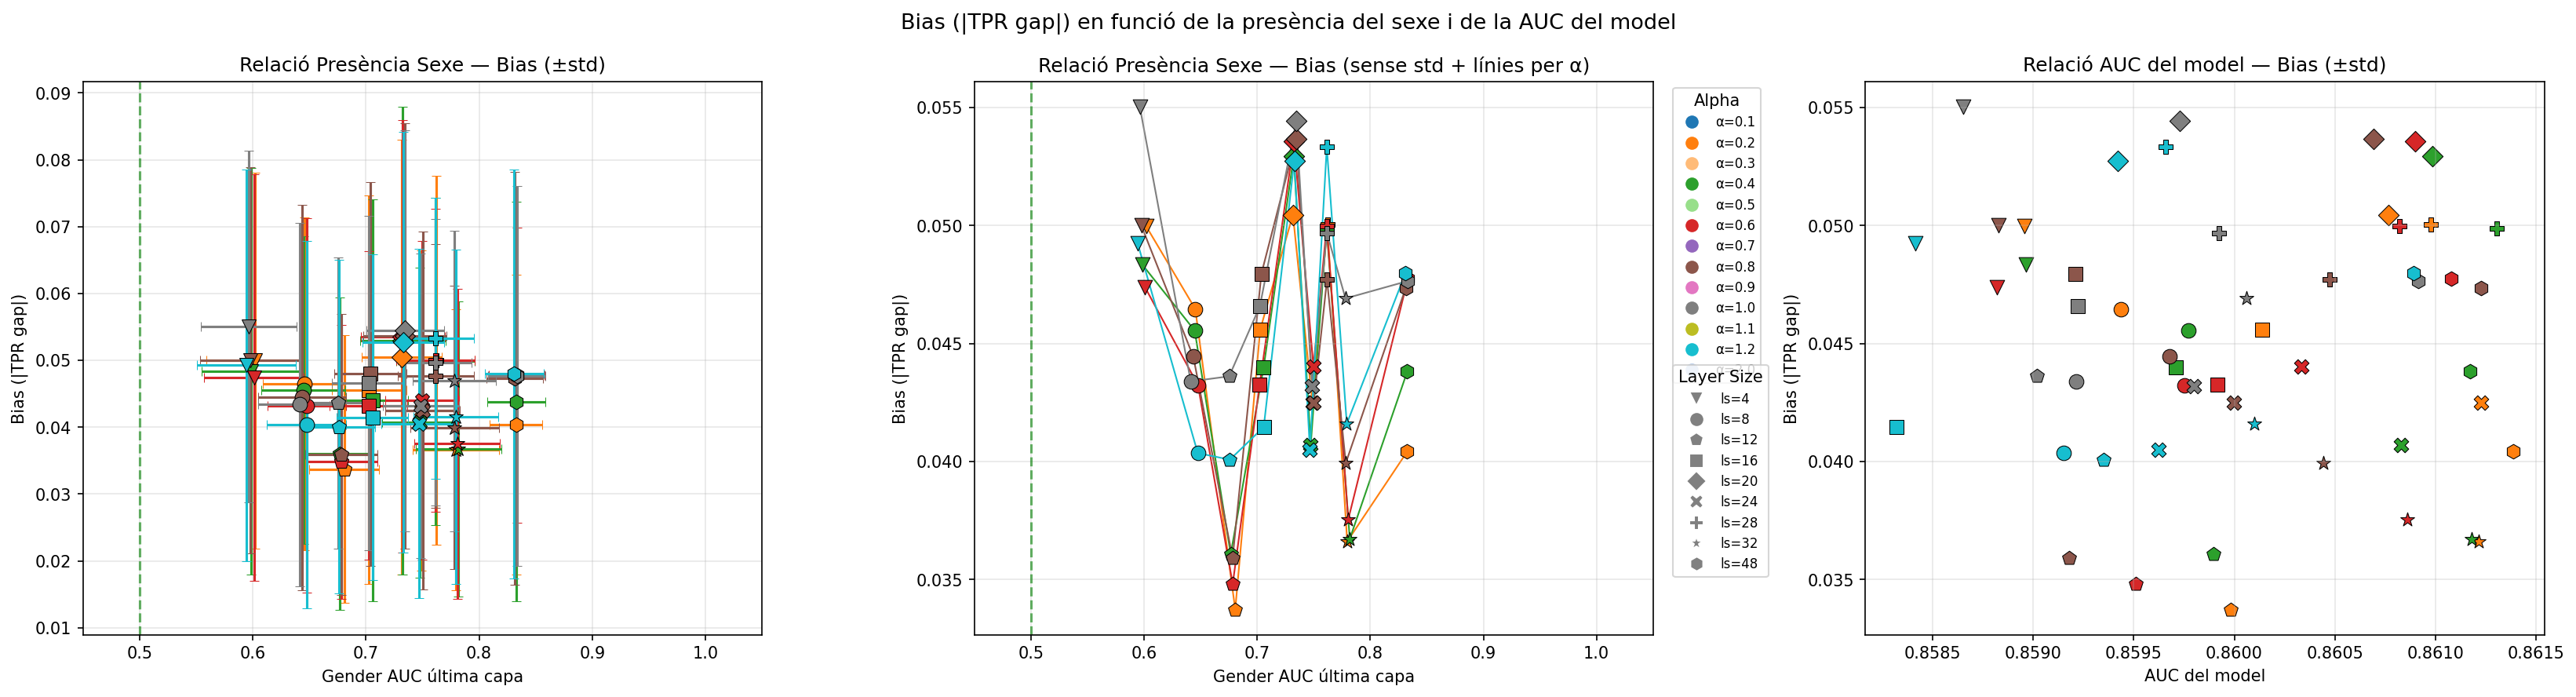
\includegraphics[width=0.95\textwidth]{../../results/sweep_bias_accuracy/20260426_025714/scatter_gender_auc_vs_model_auc_v2.png}\\[0.3em]
  {\scriptsize Les 6 condicions d'$\alpha$ se superposen en tots els panells: la variabilitat la determina $ls$.}
\end{frame}

% ── 11c. Gràfica E2 ──────────────────────────────────────────────────────────
\begin{frame}{E2 — CheXpert, $\alpha \in [0.2,\,1.2]$: penalització inerta}
  \centering
  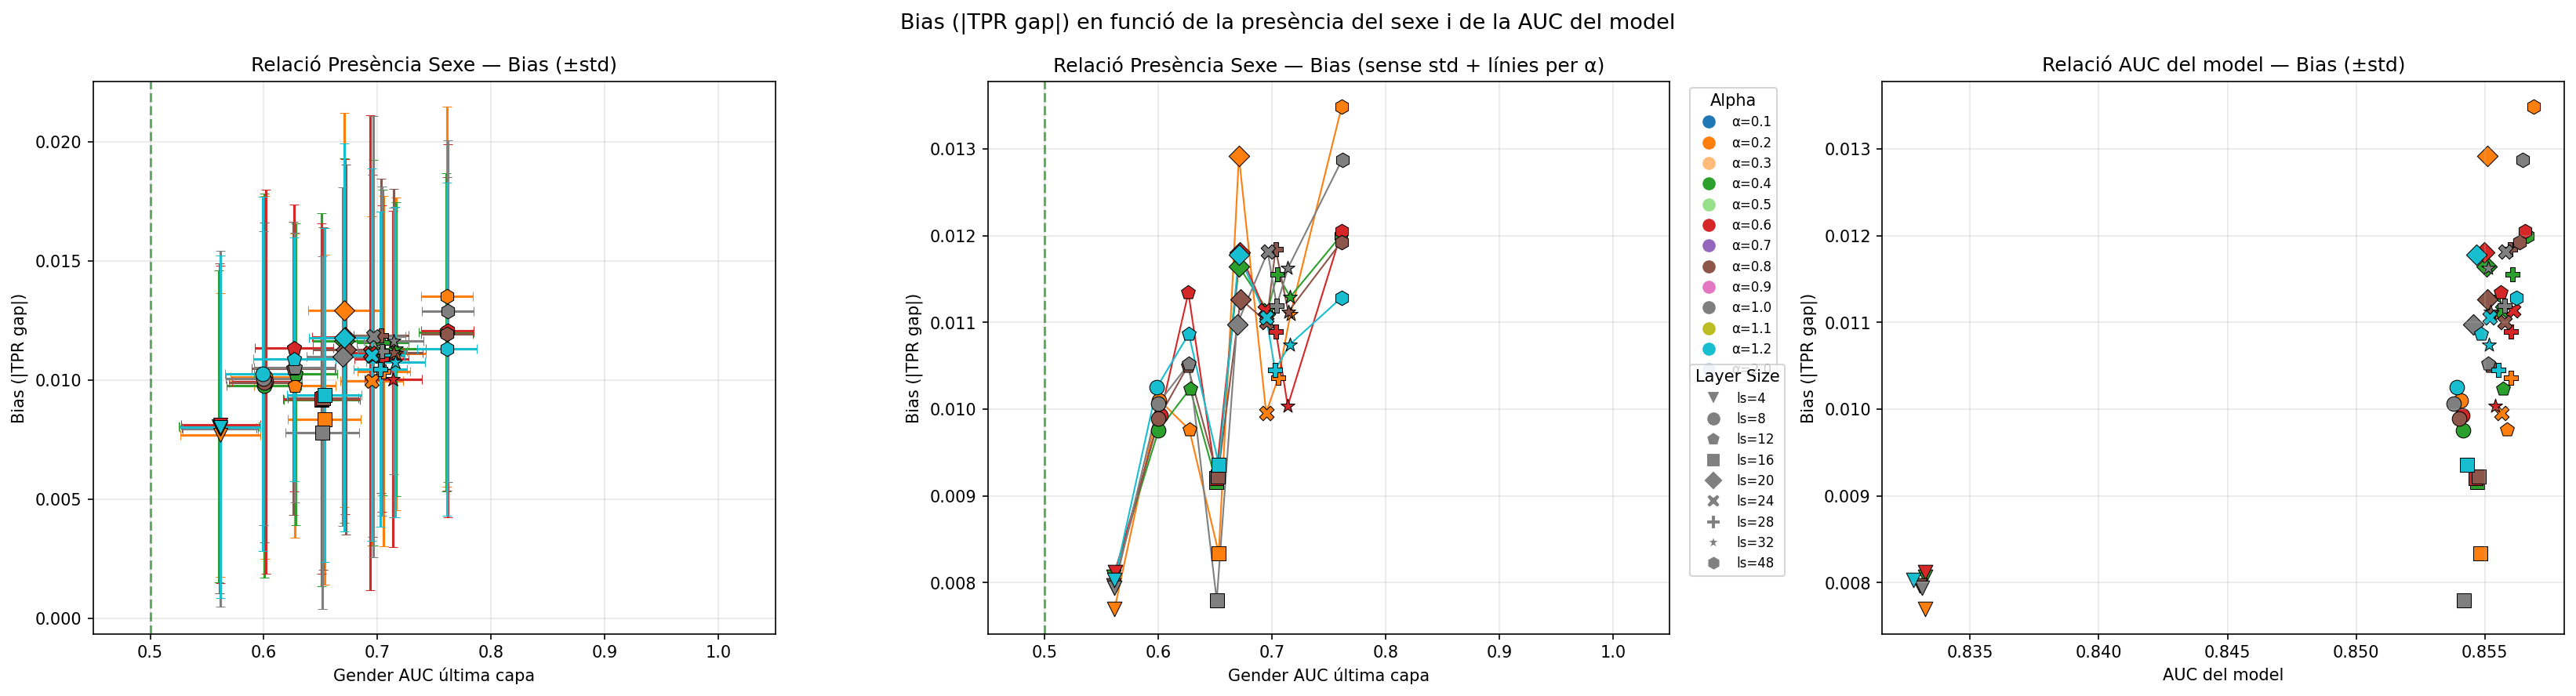
\includegraphics[width=0.95\textwidth]{../../results/sweep_bias_accuracy/20260512_035852/scatter_gender_auc_vs_model_auc_v2.png}\\[0.3em]
  {\scriptsize Idèntic patró al NIH. Biaix de partida 4 vegades menor ($\gap \approx 0.010$ vs.\ $0.050$).}
\end{frame}

% ── 12. Resultat 2 ────────────────────────────────────────────────────────────
\begin{frame}{Resultat 2: Trade-off Equitat–Precisió a $\alpha$ Alt}
  \begin{columns}[T]
    \begin{column}{0.55\textwidth}
      \textbf{En experiments E3 i E4 ($\alpha \in [1, 1000]$):}

      \smallskip
      Es detecta un \textbf{llindar crític}:
      \begin{itemize}
        \item NIH: $\alpha^* \approx 25$--$50$
        \item CheXpert: $\alpha^* \approx 10$--$25$
      \end{itemize}

      \vspace{0.3em}
      \begin{tabular}{lcc}
        \toprule
        & $\auc$ diag. & $\gap$ \\
        \midrule
        $\alpha = 0$   & 0.857 & 0.050 \\
        $\alpha = 50$  & 0.682 & 0.010 \\
        $\alpha = 1000$& 0.525 & $\approx 0$ \\
        \bottomrule
      \end{tabular}
      {\footnotesize (NIH ChestX-ray)}
    \end{column}
    \begin{column}{0.42\textwidth}
      \begin{alertblock}{Transició abrupta}
        Per sobre del llindar, el model \alert{abandona} la tasca de diagnòstic per prioritzar l'equitat.
      \end{alertblock}

      \vspace{0.5em}
      \begin{block}{Implicació}
        No hi ha \emph{gratuïtat}: aconseguir equitat real requereix sacrificar precisió diagnòstica de forma significativa.
      \end{block}
    \end{column}
  \end{columns}
\end{frame}

% ── 12b. Gràfica E3 ──────────────────────────────────────────────────────────
\begin{frame}{E3 — NIH ChestX-ray, $\alpha \in [1,\,1000]$: llindar crític visible}
  \centering
  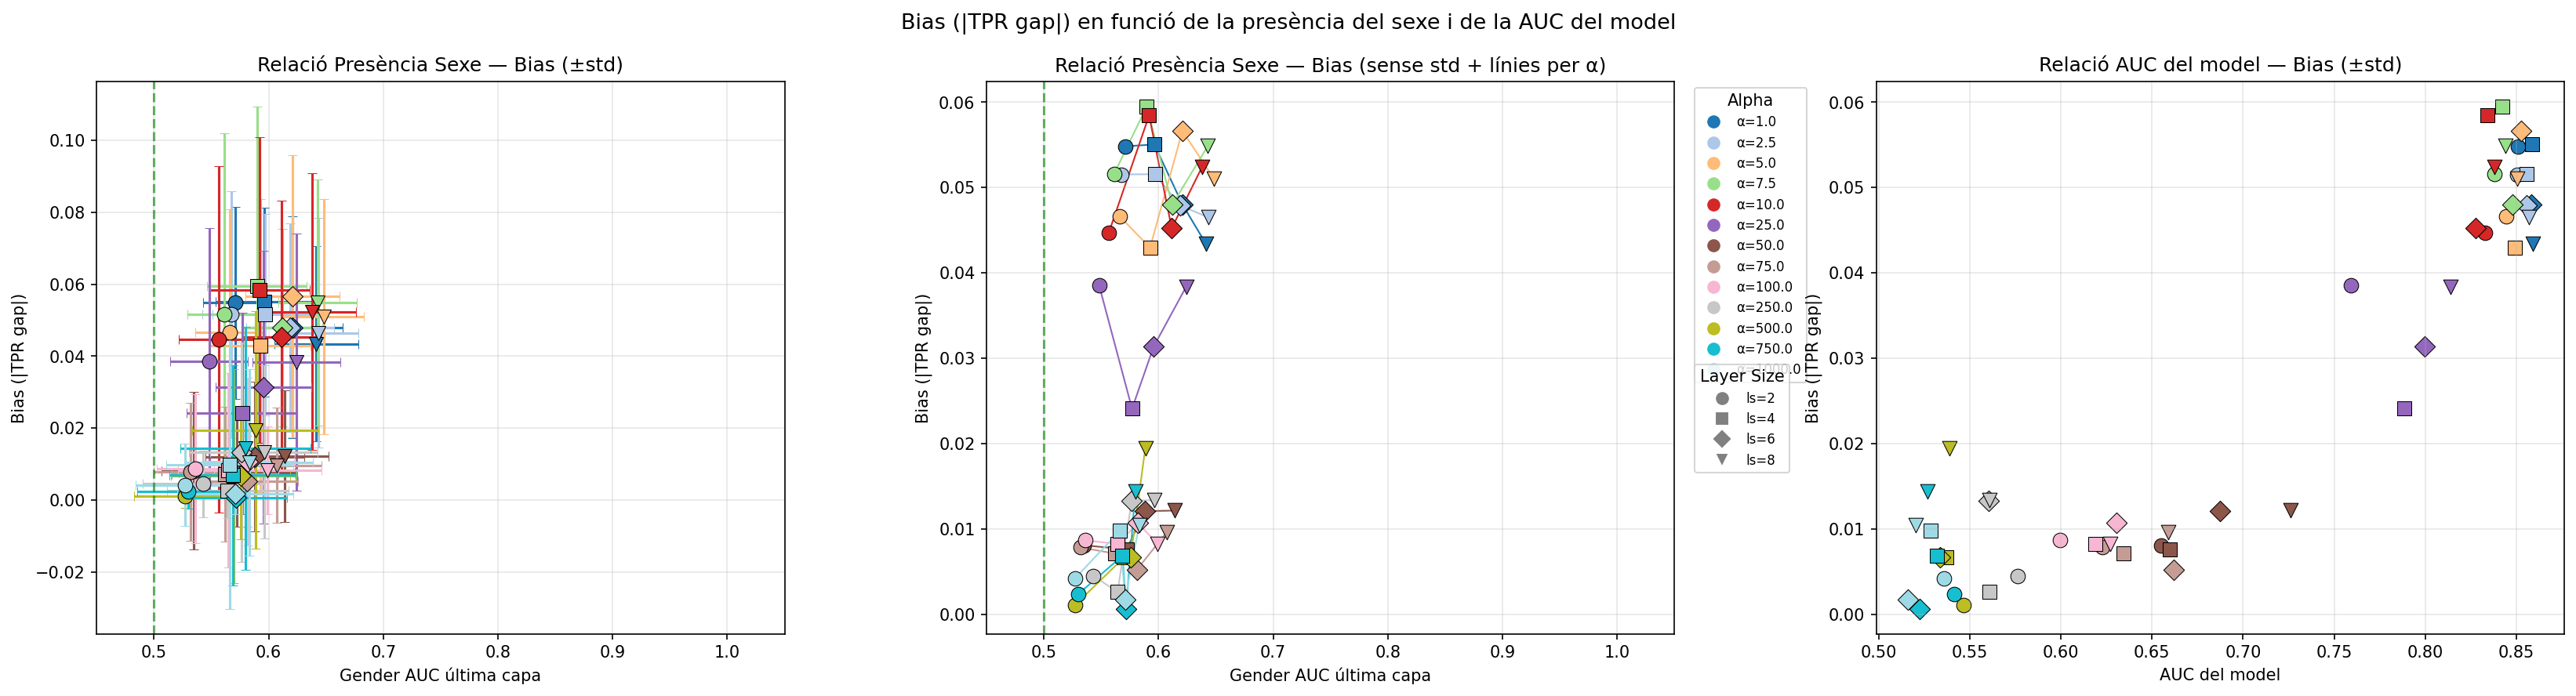
\includegraphics[width=0.95\textwidth]{../../results/sweep_bias_accuracy/20260513_195608/scatter_gender_auc_vs_model_auc_v2.png}\\[0.3em]
  {\scriptsize Panel dret: $\alpha$ creixent desplaça de dalt-dreta (alta AUC, alt biaix) cap a baix-esquerra. El llindar és \alert{visible}.}
\end{frame}

% ── 12c. Gràfica E4 ──────────────────────────────────────────────────────────
\begin{frame}{E4 — CheXpert, $\alpha \in [1,\,1000]$: llindar crític anterior}
  \centering
  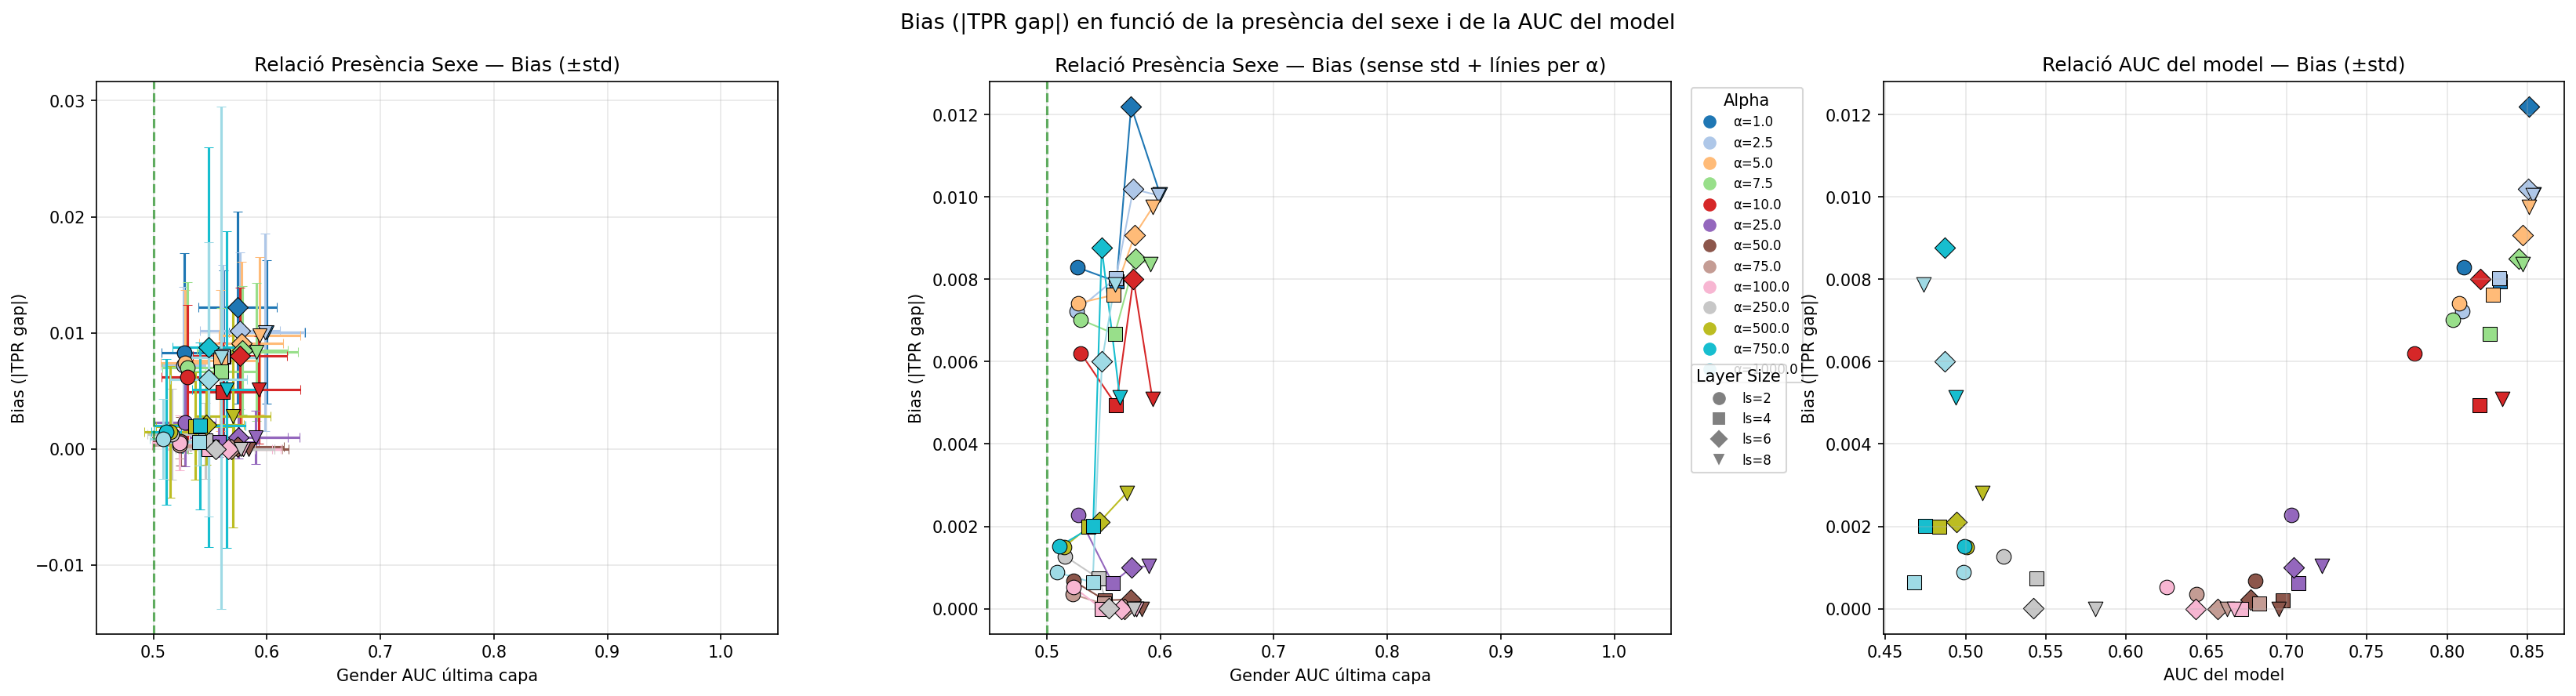
\includegraphics[width=0.95\textwidth]{../../results/sweep_bias_accuracy/20260513_195713/scatter_gender_auc_vs_model_auc_v2.png}\\[0.3em]
  {\scriptsize El llindar arriba abans al CheXpert ($\alpha^{*}\!\approx\!10$--$25$ vs.\ $\approx\!100$ al NIH).}
\end{frame}


% ── 14. Resum de resultats ────────────────────────────────────────────────────
\begin{frame}{Resum de Resultats}
  \begin{center}
  \renewcommand{\arraystretch}{1.4}
  \begin{tabular}{@{}c p{0.86\textwidth}@{}}
    \toprule
    & \textbf{Troballa} \\
    \midrule
    \textbf{R1} & Penalitzacions febles ($\alpha < 1.2$) no redueixen el biaix ni la codificació de gènere \\
    \textbf{R2} & Existeix un llindar crític $\alpha^*$ on l'equitat es compra a costa de la precisió diagnòstica \\
    \textbf{R3} & $ls$ és el principal determinant de la codificació; el backbone presenta $\auc \approx 1.0$ sempre \\
    \textbf{R4} & Els patrons qualitatius es repliquen entre NIH i CheXpert; les pràctiques del dataset impacten l'equitat tant com l'algorisme \\
    \bottomrule
  \end{tabular}
  \end{center}
\end{frame}

% ══════════════════════════════════════════════════════════════════════════════
\section{Conclusions}

% ── 16. Respostes a les RQ ───────────────────────────────────────────────────
\begin{frame}{Respostes a les Preguntes de Recerca}
  \begin{description}[\textbf{RQ3}]
    \setlength\itemsep{0.8em}
    \item[\textbf{RQ1}] \textcolor{green!50!black}{\textbf{Sí.}} El gènere es codifica internament en totes les capes analitzades, inclosa la capa densa.

    \item[\textbf{RQ2}] \textcolor{green!50!black}{\textbf{Sí.}} Una capa densa ($ls$) més gran permet recombinar la informació del backbone i augmenta la decodificabilitat lineal del gènere de forma monòtona.

    \item[\textbf{RQ3}] \textcolor{orange!80!black}{\textbf{No de forma consistent.}} La penalització d'equitat no incrementa la codificació de gènere — és la capacitat $ls$ qui la determina. La hipòtesi paradoxal no es confirma.
  \end{description}
\end{frame}

% ── 17. Contribucions i implicacions ─────────────────────────────────────────
\begin{frame}{Contribucions i Implicacions Pràctiques}
  \begin{columns}[T]
    \begin{column}{0.52\textwidth}
      \textbf{Contribucions principals:}
      \begin{itemize}
        \setlength\itemsep{0.4em}
        \item Anàlisi sistemàtica capa a capa de la codificació de gènere sota restriccions d'equitat
        \item Identificació del llindar crític on la penalització passa d'inerta a destructiva
        \item Evidència que la capacitat del model ($ls$), no la penalització, domina la codificació
      \end{itemize}
    \end{column}
    \begin{column}{0.46\textwidth}
      \textbf{Implicacions per a la pràctica:}
      \begin{itemize}
        \setlength\itemsep{0.4em}
        \item Penalitzacions febles \alert{no serveixen}: cal $\alpha$ gran
        \item Penalitzacions fortes \alert{requereixen sacrificar} precisió diagnòstica
        \item La codificació de gènere persisteix fins i tot amb $\alpha$ molt alt
        \item La qualitat i diversitat del \textbf{dataset és decisiva}
      \end{itemize}
      \vspace{0.3em}
      \begin{alertblock}{Paradoxa de privacitat}
        Models dissenyats per ser equitatius codifiquen activament el gènere internament.
      \end{alertblock}
    \end{column}
  \end{columns}
\end{frame}

% ── 18. Limitacions i treball futur ──────────────────────────────────────────
\begin{frame}{Limitacions i Treball Futur}
  \begin{columns}[T]
    \begin{column}{0.48\textwidth}
      \textbf{Limitacions:}
      \begin{itemize}
        \item Biaixos intrínsecs baixos en ambdós datasets; cal validar en contexts amb major disparitat
        \item El linear probing detecta únicament codificació \emph{lineal}; encodings no lineals podrien escapar-hi
        \item La mètrica Gap TPR no és l'única mesura d'equitat rellevant
      \end{itemize}
    \end{column}
    \begin{column}{0.48\textwidth}
      \textbf{Treball futur:}
      \begin{itemize}
        \item Altres atributs protegits: ètnia, edat, tipus d'escàner
        \item Mètodes d'anàlisi no lineals: MMD, HSIC
        \item Validació clínica amb radiòlegs
        \item Datasets amb major disparitat (MIMIC-CXR)
      \end{itemize}
    \end{column}
  \end{columns}
\end{frame}

% ── 19. Gràcies ───────────────────────────────────────────────────────────────
\begin{frame}[plain]
  \begin{center}
    \vspace{1.5cm}
    {\Large\textbf{Gràcies per la vostra atenció}}\\[1.5em]
    {\large Joan Massallé Richart}\\[0.5em]
    {\normalsize Màster en Ciència de Dades — EPS, Universitat de Girona}\\[0.5em]
    {\normalsize Juny 2026}\\[2em]
    \rule{0.6\textwidth}{0.4pt}\\[1em]
    {\normalsize\textit{Tutor: Jerónimo Hernández González}}
  \end{center}
\end{frame}

\end{document}
